\section{The initial representation-learning programme}
\label{sec:early}

PHASE-TTC began as E-JEPA-TTC, a study of predictive event representations for time-to-contact estimation. The programme covered pooled and spatial embeddings, apparent expansion, and transport-conditioned residual dynamics. Some models improved TTC while losing the geometric behaviour that motivated them, so the experiments assessed accuracy, geometric consistency, and representation content separately.

The historical names distinguish otherwise similar version numbers. \emph{Causal Scale v5--v8} refers to synthetic operator tests, whereas \emph{Scientific Recovery V5--V8} refers to later real-data studies. The EvTTC and eAP A0/A1 experiments also used different data and metrics.

\begin{figure}[htbp]\centering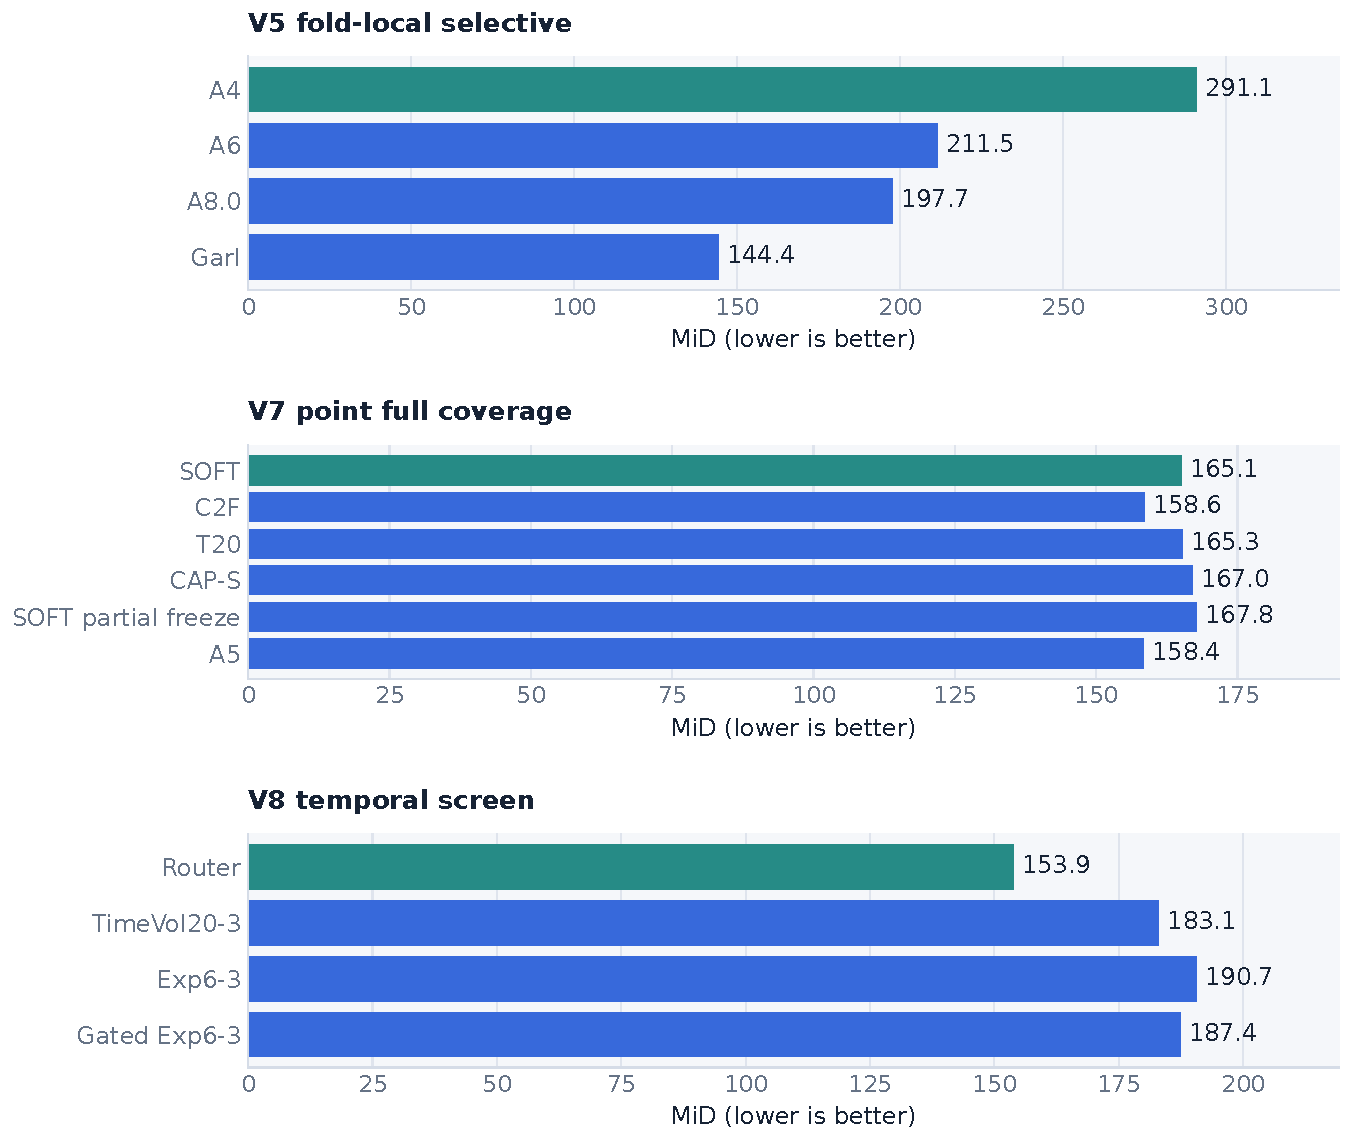
\includegraphics[width=\linewidth]{figures/early_ablation.pdf}
\caption{Early recovery results by experiment family; lower MiD is better.}\label{fig:early}
\end{figure}

\subsection{Global and dense representations on EvTTC}

Global A0 remained preferable to Dense A1 in the matched EvTTC comparison. Five grouped folds and seeds 7, 13, and 21 produced fifteen paired runs per model (Table~\ref{tab:early-evttc}). \evidence{E01}

\begin{table}[htbp]
\centering\small
\begin{tabular}{lrrr}
\toprule
Architecture & MAE (s) & Relative error (\%) & Selection score \\
\midrule
Global A0 & 1.0109 & 30.25 & 0.58452 \\
Dense A1 & 1.0067 & 30.55 & 0.59312 \\
\bottomrule
\end{tabular}

\caption{Global A0 and Dense A1 means over five EvTTC folds and three seeds.}
\label{tab:early-evttc}
\end{table}

Dense A1 reduced mean absolute error, but increased both relative error and the registered composite selection score. It also used 2.16 times A0's measured latency and 1.58 times its training time. We retained the smaller global model. \evidence{E01}

Attention residuals, temporal KDA/Object-KDA, object-conditioned crops, and FlowMimic-style alignment all failed their selection gates. Because those screens used different data or criteria, they do not extend the matched A0/A1 ranking.

\subsection{Representation variance and dynamic information}

The temporal-residual objective captured the desired dynamics under a slow synthetic nuisance process. Its mean dynamic $R^2$ was about $0.72$, versus $0.15$ for variance regularization. The latter maintained high embedding variance while preserving nuisance information, showing that variance alone was a poor proxy for useful temporal content. \evidence{E02}

Changing the nuisance on every frame reversed the result: the residual objective's dynamic $R^2$ became negative, while the variance control reached about $0.74$. Later probes kept both level and change features and varied the nuisance process. Neither effective rank nor per-dimension standard deviation demonstrated TTC-relevant content on its own. \evidence{E02,E12}

\subsection{Object identity and crop geometry}

Object-level eAP/GarlTTC requires an explicit query because several annotated objects can share one event frame while having different TTC values. Object-LHR resolved the ambiguity by cropping the selected object at both endpoints before estimating temporal scale.

Independent resizing erased much of the apparent scale change required by the geometric head. Object-Expansion v2 stabilized the output by predicting sign and log inverse-TTC magnitude; Object-Signed-Expansion v3 combined them in one expansion coordinate and added ordered temporal features plus box motion. Perturbation tests showed strong dependence on box motion and little response to events, so this accuracy could not be credited to event representation learning.

Object Event v4 placed three causal endpoints in one common crop, preserving apparent growth and separating the neural event path from the motion ablation. The object query and its coordinate system became part of the model specification. Earlier variants used different conditions and remain separate experiments.

\subsection{Physical tests of the scale operator}

The frozen v4.31 matcher passed representation-stability checks but failed the zoom, reversal, and translation requirements. We also found uncommitted source changes and a missing evidence stage, so the run was ineligible for selection. Its foreground, height, pseudoflow, and correspondence diagnostics motivated a new scale estimator.

For two apparent heights $h_{t-1}$ and $h_t$ separated by $\Delta t$, the Causal Scale operator defines
\begin{equation}
 r_t=\log h_t-\log h_{t-1},\qquad
 \widehat{\tau_t^{-1}}=\frac{\exp(r_t)-1}{\Delta t}.
 \label{eq:early-scale}
\end{equation}
Under idealised constant-speed approach, this gives inverse TTC at the newer endpoint. Changes in shape, viewpoint, occlusion, or relative motion can violate the geometric assumptions. For $\hat\tau_t=\Delta t/(\exp(r_t)-1)$, the sensitivity is
\begin{equation}
 \frac{\partial\hat\tau_t}{\partial r_t}
 =-\frac{\Delta t\exp(r_t)}{(\exp(r_t)-1)^2}.
\end{equation}
The derivative grows without bound as $r_t$ approaches zero. Output clipping can contain the resulting TTC value, but it cannot improve the scale measurement.

The learned foreground failed to reproduce the ideal operator on held-out synthetic data. Causal Scale v5 reached correlation $0.92$ with translation leakage $0.027$, missing both requirements. V7 reduced leakage to $0.0034$ and symmetric TTC error to $0.25$, but correlation stayed at $0.92$ and the validation result did not transfer to the new synthetic group. \evidence{E13,E14}

Causal Scale v8 selected on both mean and worst-group performance across independent synthetic groups. Fixed symmetric smoothing supported sparse endpoints, and a final CVaR loss emphasized large ratio errors. Correlation remained below the gate in every group. We nevertheless continued to a real-data screen, treating it as exploratory. \evidence{E15}

\subsection{Foreground supervision in the first eAP screens}

The first eAP screens used a common object crop, three event endpoints, and oracle boxes; they did not evaluate detection. A0 learned a weak rectangular foreground target. A1 replaced it with height, width, and centre supervision. A1-FR added a full-resolution decoder, A1-DF used deeper features, and A1-DF-R supervised the pair ratio directly. A3 kept the A1 architecture and trained with RGB-derived SAM masks. All screens reused public validation data.

\begin{table}[htbp]
\centering\small
\begin{tabular}{lrr}
\toprule
Arm & MiD $\downarrow$ & Failure (\%) \\
\midrule
A1 geometry & 346.829 & 9.961 \\
A3 SAM distilled & 353.635 & 10.889 \\
Garl trained matched & 203.634 & 0.000 \\
\bottomrule
\end{tabular}

\caption{Early eAP public-validation results for A0, A1, A3, and matched Garl.}
\label{tab:early-screen}
\end{table}

A3 did not improve on A1, and both scored worse in aggregate MiD than matched Garl. The diagnostics showed that estimating absolute height did not guarantee recovery of its temporal derivative. Garl achieved lower aggregate error but predicted positive TTC for receding cases, leaving signed motion unresolved. \evidence{E25,E26}

A4 distilled local spatial relations from a frozen DINOv3 RGB teacher into an event student; A4D also learned changes in those relations across endpoints. Both used RGB during training and events at inference. A5 and A6 then varied TTC specialization and transport while monitoring the inherited geometry.

\subsection{Scientific Recovery V5: fold-specific producer training}

The first grouped-development run inherited an A4 parent trained on all nine development sequences, including each held-out outer group. We excluded it from promotion and retrained A4 inside every outer fold. The corrected study initialized A6 and A8.0 from the matching fold-local parent and trained Garl from scratch. \evidence{E03}

The comparison matched samples, targets, training budget, metric, and oracle-ROI access. The E-JEPA-family branch used three endpoints and twelve channels; Garl used two endpoints and forty channels. Checkpoint selection still used the outer-development split, and TTC buckets shaped the initial 8,192-token sample. Thus, the correction removed parent exposure without turning the study into a blind test or a target-free sample. \evidence{E03}

\begin{table}[htbp]
\centering\small
\begin{tabular}{lrrr}
\toprule
Model & Parameters & MiD $\downarrow$ & Failure (\%) \\
\midrule
A4 parent & 355,118 & 291.088 & 9.448 \\
A6 transport & 498,130 & 211.509 & 7.849 \\
A8.0 dual transport & 627,827 & 197.691 & 7.019 \\
V6.1 radius 2 & 627,827 & 194.122 & 6.689 \\
A5 causal & 424,274 & 155.472 & 4.761 \\
Garl local matched & 24,674,178 & 144.353 & 0.000 \\
\bottomrule
\end{tabular}

\caption{Scientific Recovery V5--V6 results on 8,192 tokens from nine sequences, three folds, and seed 7.}
\label{tab:early-v5v6}
\end{table}

A8.0, which freed transport while retaining the frozen parent geometry, improved MiD over A6 by 13.8 points; the paired 95\% interval was $[-17.7,-10.1]$. It still exceeded the preregistered MiD threshold of 175 and remained behind Garl, so V5 produced no candidate. \evidence{E03,E05}

Sequence-scoped track identifiers and preserved token/target IDs made the fold-local correction auditable through the full training lineage.

\subsection{Scientific Recovery V6--V7: accuracy and geometric retention}

Increasing the transport radius from one to two did not yield a clear V6 gain: V6.1 reduced mean MiD relative to A8.0, but the paired interval $[-8.2,1.0]$ crossed zero. A5 achieved lower TTC error than the geometry-frozen variants while weakening their geometric dynamics, which kept accuracy and mechanism retention as separate criteria. \evidence{E04,E06}

V7 tested soft geometric distillation, coarse-to-fine transport, extra temporal bins, greater capacity, and partial freezing. Under full-coverage point evaluation, A5 scored 158.4 MiD and served as the reference. Promotion required both lower TTC error and retained geometric behaviour. \evidence{E07,E08,E09,E10,E11}

\begin{table}[htbp]
\centering\small
\begin{tabular}{lrrr}
\toprule
Arm & Point MiD & Delta vs A5 & Paired 95\% interval \\
\midrule
A5 reference & 158.449 & -- & -- \\
SOFT & 165.116 & +6.668 & [+3.084, +10.547] \\
C2F & 158.573 & +0.125 & [-3.025, +3.432] \\
T20 & 165.260 & +6.812 & [+2.290, +11.514] \\
CAP-S & 167.025 & +8.576 & [+3.735, +13.630] \\
SOFT partial freeze & 167.826 & +9.378 & [+5.359, +13.272] \\
\bottomrule
\end{tabular}

\caption{V7 full-coverage MiD relative to A5, using seed 7 and three outer folds.}
\label{tab:early-v7}
\end{table}

Every V7 arm failed at least one mechanism, geometry, or confirmation gate, and none advanced to confirmation seeds. More temporal bins, capacity, and partial freezing did not close the comparator gap. The JEPA objective was inactive in these runs, so their results provide no evidence about JEPA pretraining. \evidence{E07,E08,E09,E10,E11}

A post-hoc A5/C2F analysis found complementary errors. We separated a deployable feature-based router from a target-aware oracle and used the result only to design V8's prospective nested-routing test.

\subsection{Scientific Recovery V8: nested routing and JEPA attribution}

Only the nested A5/C2F router passed V8's candidate screen; all three temporal-representation interventions failed it. \evidence{E16,E17,E18,E19}

\begin{table}[htbp]
\centering\small
\begin{tabular}{lrrr}
\toprule
Arm & MiD & Finite (\%) & Stored gate \\
\midrule
router & 153.877 & 100.00 & True \\
timevol20\_3 & 183.092 & 95.25 & False \\
exp6\_3 & 190.711 & 94.10 & False \\
gated\_exp6\_3 & 187.400 & 94.80 & False \\
\bottomrule
\end{tabular}

\caption{V8 seed-7 MiD and finite coverage for the router and temporal-representation arms.}
\label{tab:early-v8}
\end{table}

The seed-7 router improved on A5 by 4.6 MiD points. Its scores were 153.9, 153.3, and 156.0 for seeds 7, 13, and 23. All three runs reused the same development sequences and estimate optimization stability, not independent external replication. Matched Garl seed replications were unavailable. \evidence{E16,E20}

The stored V8 summaries support point estimates, finite coverage, and gate outcomes. They do not specify enough aggregation detail to reconstruct valid uncertainty intervals, so none are reported.

A post-training path replay located the trained model's dependence. The analytic height path had high error, and adding a residual without transport changed little. Transport plus the residual produced the main improvement; history added a smaller gain. Because the replay disabled paths without retraining, it measures use inside this trained graph rather than the effect of retraining each ablation. \evidence{E21}

\begin{table}[htbp]
\centering\small
\begin{tabular}{lr}
\toprule
Replay intervention & MiD $\downarrow$ \\
\midrule
analytic only & 373.176 \\
analytic residual & 373.596 \\
analytic residual transport & 163.231 \\
analytic residual transport history & 155.824 \\
analytic transport & 373.176 \\
\bottomrule
\end{tabular}

\caption{V8 post-training path replay showing MiD for the analytic, residual, transport, and history paths.}
\label{tab:early-factorial}
\end{table}

The H2 diagnosis was shortcut/residual dominance: the analytic height path did not explain the trained model's advantage. We next tested a measurement interface with less dependence on explicit height estimation. The diagnosis did not rule out useful geometry or transport features. \evidence{E22}

V8 tested JEPA attribution through D0--D4. The meta-router had no single transferable encoder, so A5 supplied the downstream reference. D2 froze the JEPA encoder, D3 fine-tuned part of it, and scratch, random-frozen, and shuffled-future arms controlled for downstream capacity and temporal correspondence. \evidence{E24}

\begin{table}[htbp]
\centering\small
\begin{tabular}{lrrrrr}
\toprule
Arm & 1\% & 5\% & 10\% & 25\% & 100\% \\
\midrule
D2 & 379.95 & 379.88 & 379.94 & 379.79 & 379.99 \\
D3 & 379.52 & 379.38 & 379.39 & 379.32 & 379.67 \\
\bottomrule
\end{tabular}

\caption{V8 JEPA attribution across nominal label fractions for D0--D4.}
\label{tab:early-jepa}
\end{table}

D2 and D3 produced finite predictions with no recorded failures, but neither passed the causal-benefit gate against scratch, random-frozen, and shuffled-future controls. V8 provided no positive JEPA attribution, and the next experiments focused on the measurement interface and feature usefulness. \evidence{E23}
